%\documentclass[a4paper, twocolumn]{article}
\documentclass[a4paper,11pt]{article}
\usepackage{multicol}
\usepackage{calc}
\usepackage{ifthen}
\usepackage[margin=1cm,top=0.1cm,left=0.01cm,right=0.1cm,bottom=0.2cm, nohead,nofoot]{geometry}

\usepackage{mdwlist} % Avoid list double spacing

\usepackage[usenames,dvipsnames]{color}
\newcommand\todo[1]{\textcolor{red}{#1}}

% Turn off header and footer
\pagestyle{empty}
%\usepackage{enumitem}
\usepackage[shortlabels]{enumitem}
\setlist{leftmargin=0.5cm,itemsep=0pt,topsep=0pt,partopsep=0pt,parsep=0pt}

\usepackage[compact]{titlesec}
\titleformat{\section}{\normalfont\normalsize\bfseries\color{BlueViolet}}{\thesection}{1em}{}
\titleformat{\subsection}{\normalfont\small\bfseries\color{blue}}{\thesubsection}{1em}{}
\titleformat{\subsubsection}{\normalfont\small\bfseries\color{cyan}}{\thesubsubsection}{1em}{}
%\titleformat{\paragraph}{\normalfont\small\bfseries\color{black}}{\theparagraph}{1em}{}
\titleformat*{\paragraph}{\small\bfseries}

\titlespacing*{\section}{0pt}{*0}{0pt}
\titlespacing*{\subsection}{0pt}{*0}{0pt}
\titlespacing*{\subsubsection}{0pt}{*0}{0pt}

% Define BibTeX command
\def\BibTeX{{\rm B\kern-.05em{\sc i\kern-.025em b}\kern-.08em
    T\kern-.1667em\lower.7ex\hbox{E}\kern-.125emX}}

% Don't print section numbers
\setcounter{secnumdepth}{0}

\setlength{\parindent}{0pt}
\setlength{\parskip}{0pt plus 0.5ex}

% math packages
\usepackage{amsmath}
\usepackage{amsfonts} % for mathbb for instance
\usepackage{mathtools}
\usepackage[amsmath, amsthm, framed, thmmarks]{ntheorem}

% specifics about the pdf
\usepackage[utf8]{inputenc}
\usepackage[english]{babel}
\usepackage[pdftex]{graphicx}
\usepackage[pdftex,bookmarks,colorlinks,pdffitwindow]{hyperref}

\usepackage[letterspace=-4]{microtype}

% for indent
\usepackage{scrextend}

% for rotating table
\usepackage{rotating}


\usepackage{setspace}
\renewcommand{\baselinestretch}{1}  %0.2 still ok!

% redefine greek letters
\renewcommand{\phi}{\varphi}
\renewcommand{\epsilon}{\varepsilon}

% shortcuts in math mode
\newcommand{\bs}{\boldsymbol}
\newcommand{\mc}{\mathcal}
\newcommand{\ds}{\displaystyle}
\DeclarePairedDelimiter\absimpl{\lvert}{\rvert}
\DeclarePairedDelimiter\normimpl{\lVert}{\rVert}
\newcommand{\abs}[1]{\absimpl*{#1}}
\newcommand{\norm}[1]{\normimpl*{#1}}
\newcommand{\argmax}{\operatorname*{arg\,max}}
\newcommand{\argmin}{\operatorname*{arg\,min}}

% number sets
\newcommand{\R}{\mathbb{R}}
\newcommand{\B}{\mathbb{B}}
\newcommand{\Z}{\mathbb{Z}}
\newcommand{\N}{\mathbb{N}}
\newcommand{\Q}{\mathbb{Q}}
\newcommand{\C}{\mathbb{C}}
\newcommand{\F}{\mathbb{F}}
\newcommand{\LL}{\mathcal{L}}
\newcommand{\powerset}{\mathcal P}
\newcommand{\normal}{\mathcal N}

\newcommand{\sectionline}{\noindent\makebox[\linewidth]{\rule{\columnwidth}{0.1pt}}}
\newcommand{\msection}[1]{\section{#1}\vspace{-0.5mm}}
% probabilities
\newcommand{\Prob}[1]{\operatorname{Pr}\left[#1\right]}
\newcommand{\Ex}[1]{\mathbb{E}\left[#1\right]}

% misc
\newcommand{\bigO}[1]{\mc O\left(#1\right)} % big-o notation

\newcommand{\nop}[1]{} % temporarily remove from output

\newcommand{\tf}{\text{tf(w; d)}} % tf - term frequency
\newcommand{\cf}{\text{cf(w)}} % df - collection frequency
\newcommand{\df}{\text{df(w)}} % df - document frequency
\newcommand{\idf}{\text{idf(w)}} % idf - inverse document frequency
\newcommand{\w}{\text{w}}
\newcommand{\btheta}{\boldsymbol \theta}

% remove the paragraph indentation
 \setlength{\parindent}{0in}

\begin{document}
\raggedright
\lsstyle
\small
\setlength{\columnseprule}{0.1mm}
\abovedisplayskip=0pt
\belowdisplayskip=0cm
\allowdisplaybreaks
\itemsep-0.7em
\labelsep=0.05cm

\begin{multicols}{2}

%%%%%%%%%%%%%%%%%%%%% Various %%%%%%%%%%%%%%%%%%%%%%%%%%
\section{Various}
\paragraph{Filtering (Stop word removal):} Get grid of common terms\\
+ reduce vocabulary size (space), - language specific

\paragraph{Stemming:} Stripping off word endings to reduce a word to its stem/core (e.g. PorterStemmer).
\begin{itemize}[leftmargin=0.3cm]
  \item [+] reduce vocabulary size (space)
  \item [+] unifies words with same meaning, but slight variation (foxes $>$ fox)
  \item [--] language specific (for each language different rules)
  \item [--] 1 extra step (quite expensive)
  \item [--] can result in non-dictionary words
  \item [--] words with different meaning can be mapped to same word (automatic / automate $>$ autom)
\end{itemize}

\paragraph{Lemmatization:} Mapping words to its root form. \\
E.g. (walk, walked, walks, walking) $>$ walk or better $>$ good\\
+ get true dictionary form of a word, - hard to achieve in practice

\paragraph{Term normalization (general):} Allows matching more terms\\
\begin{itemize}[leftmargin=0.3cm]
  \item [+] identify small variations of same term
  \item [--] can lead to loss in precision
\end{itemize}

%%%%%%%%%%%%%%%%%%%%% Evaluation of Relevance %%%%%%%%%%%%%%%%%%%%%%%%%%
\msection{3 - Evaluation of Relevance}
\paragraph{Precision (P):} Fraction of retrieved documents that are relevant.
\[
  \text P = \frac{\# \text{ relevant items retrieved}}{\# \text{ items retrieved}} 
          = \frac{\text{TP}}{\text{TP + FP}}
          %= P(\text{X is relevant} | \text{X is retrieved})
\]

\paragraph{Recall (R):} Fraction of relevant documents that are retrieved.\\
\[
  \text R = \frac{\# \text{ relevant items retrieved}}{\# \text{ relevant items in collection}}
          = \frac{\text{TP}}{\text{TP + FN}}
          % P(\text{X is retrieved} | \text{X is relevant}) 
\]
\\
\vspace{0.2cm}
\textcolor{red}{High Precision vs High Recall:} It's a tradeoff!
\begin{itemize}
  \item By returning more documents $\Rightarrow$ recall increases monotonically\\
        E.g. return all document $\Rightarrow$ recall of 1\\
        \underline{Comparison shopping} $\Rightarrow$ wants high recall (user wants all offers)
  \item By returning fewer documents $\Rightarrow$ often precision increases\\
        E.g. return 1 document $\Rightarrow$ precision of 1 \underline{if} document is relevant\\
        \underline{Web search} $\Rightarrow$ wants high precision (user just looks at few result)
\end{itemize}

\paragraph{F-Measure (F):} Something in between precision and recall
\begin{align*}
  F_{\beta} &= \frac{(\beta^2 + 1) \text{PR}}{\beta^2 \text P + \text R} \hspace{0.3cm} \text{where } \beta^2 = \frac{1 - \alpha}{\alpha} \\
  F_1 &= \frac{2 \; \text{PR}}{\text{P + R}}
\end{align*}

\paragraph{A/B tests:} Can also run A/B tests with 2 systems\\
\begin{enumerate}
  \item Sample queries to evaluate on 2 systems
  \item For each query show both results to raters
  \item Raters judge which system is better
  \item Compute overall statistics
\end{enumerate}

%%%%%%%%%%%%%%%%%%%%% Scoring: TF-IDF %%%%%%%%%%%%%%%%%%%%%%%%%%
\msection{4 - Scoring: TF-IDF}
\paragraph{Scoring by matching terms:} We have the general expectation:
\begin{itemize}[leftmargin=0.3cm]
  \item If query term doesn't occur in document $\Rightarrow$ score contribution should be 0! 
  \item The more frequent the query term in the document $\Rightarrow$ the higher the score contribution!
  \item The more informative the query term $\Rightarrow$ the higher the score contribution! E.g. bomb
  \item Given same term frequency $\Rightarrow$ shorter document should be preferred
\end{itemize}

\paragraph{Term Frequency:} Absolute frequency of a word in a document
\begin{align*}
  \tf =& \# \text{ word w in document d}\\
  \text{log-tf(w; d)} =& \log_2\left(1 + \frac{\tf}{\text{document\_length}} \right)\\
  \text{atf(w; d)} =& \frac{1}{2} + \frac{1}{2} \frac{\tf}{\max\{ \text{w}' : \text{tf(w$'$; d)} \}} \\
  \text{score(\text{query}; d)} &= \sum_{\text w \in \text{query}} \text{log-tf(w; d)} 
\end{align*}
\textcolor{red}{Note:}
\begin{itemize}[leftmargin=0.3cm]
  \item Augmented-tf is very sensible to maximum (stop word pruning)
  \item Using raw term frequencies (tf) is discouraged in practice
\end{itemize}

\paragraph{Document Frequency:} Quantifies importance of a query term
\begin{align*}
  \df =& \; \# \{ \text d : \tf > 0\} \\
         =& \; \# \text{ documents in collection that contain w}
\end{align*}
\textcolor{red}{Note:}
\begin{itemize}[leftmargin=0.3cm]
  \item low df $\Rightarrow$ more informative/topical (e.g. bomb)
  \item high df $\Rightarrow$ less informative/topical (e.g. the)
\end{itemize}

\paragraph{Inverse Document Frequency:}\hspace{-0.3cm}Translates df into term weights\\
\begin{align*}
  \idf = \log\left(\frac{n}{\df} \right) = \log(n) - \log(\df) \hspace{0.5cm} n = \text{num documents}
\end{align*}
\textcolor{red}{Note:}
\begin{itemize}[leftmargin=0.3cm]
  \item low idf $\Rightarrow$ less informative/topical (e.g. the)
  \item high idf $\Rightarrow$ more informative/topical (e.g. bomb)
\end{itemize}

\paragraph{Collection Frequency:} Like term freq. but in whole collection
\begin{align*}
  \cf &= \sum_d \tf \\
         &= \# \text{word occurrences in whole collection}\\
  \text{rcf(w)} &= \frac{\cf}{\sum\limits_{\text{w}'} \text{cf(w$'$)}}
\end{align*}

\paragraph{TF-IDF:} Combine both tf and idf in one term weight
\begin{align*}
  \text{tf-idf(w; d)} &= \text{log-tf(w; d)} \cdot \idf \\
                      &= \log \left(1 + \frac{\tf}{\text{document\_length}} \right) \cdot \log \left( \frac{n}{\df} \right)\\
  \text{score(query; d)} &= \sum_{\text{w} \in \text{query}} \text{tf-idf(w; d)}
\end{align*}

\textcolor{red}{Note:} We want that both tf(w) and idf(w) are large!

\paragraph{Vector Space Model:} Represent both documents and queries in vector space (BoW) and rank documents according to their proximity to the query (e.g. use cosine distance).
\begin{itemize}[leftmargin=0.3cm]
  \item [+] can use linear algebra for computation
  \item [--] very high dimensional space (slows down computation)
\end{itemize}

%%%%%%%%%%%%%%%%%%%%% Scoring - LM %%%%%%%%%%%%%%%%%%%%%%%%%%
\msection{5 - Scoring: Language and Topic Model}
\subsection{Language Model}
We want to estimate the term distribution P(w$|$d) so that we can compute the query probability P(q$|$d), which can directly be used for ranking:
\begin{align*}
  \textbf{Query Likelihood: }& &\text P(\text q | \text d) &= \text P(\text w_1, ... , \text w_l | \text d) = \prod_{\text w \in \text q} \text P(\text w | \text d)\\
  \textbf{MLE: }&  &\hat{\text{P}}(\text w | \text d) &= \frac{\tf}{\sum_{\text w'} \text{tf(w$'$; d)}}\\
  \textbf{Log Q. Likelihood: }& &\text{log P}(\text q | \text d) &= \sum_{\text w \in \text q} \text{log P}(\text w | \text d) \\ 
  &&&= \sum_{\text w \in \text q} \text{log-tf(w; d)}
\end{align*}
\textbf{LM Properties:}
\begin{itemize}[leftmargin=0.3cm]
  \item [+] simple and clean model without complicated assumptions
  \item [+] can use document collection to learn these distributions
  \item [--] Assumption of query generation is too simplistic)
  \item [--] Why should relevance be tied to term distribution?
\end{itemize}
\paragraph{MLE and Smoothing:} Use smoothing to get better estimates for small frequencies (and for unseen terms).\\
E.g. linear interpolation with collection frequencies:
\begin{align*}
  \text{P(w$|$d)} &= (1 - \lambda_d) \; \hat{\text P}\text{(w$|$d)} + \lambda_d \; \underbrace{\frac{\cf}{\sum_{\text w'} \text{cf(w$'$)}}}_{\hat{\text P}(\text w)} \hspace{0.6cm} \lambda_d \in [0, 1] \\
                  &= (1 - \lambda_d) \; \hat{\text P}\text{(w$|$d)} + \lambda_d \; \hat{\text{P}} \text{(w)}
\end{align*}
\textcolor{red}{Note:} Smoothing helps to alleviate problems with small frequencies

\subsection{Topic Model}
Topic Models are statistical models trained from the document collection. The idea is to identify topics and model documents as topic mixtures. This is a latent variable model, where the topics are the latent factors. 
\begin{align*}
  \text{P(w$|$d)} = \sum_t \text{P(w$|$t)} \text{P(t$|$d)}
\end{align*}

%%%%%%%%%%%%%%%%%%%%% Text Categorization %%%%%%%%%%%%%%%%%%%%%%%%%%
\msection{6 - Text Categorization}
\paragraph{Task:} The primary task is to assign topics/categories to each text/document. But there are different types of this task:
\begin{itemize}
  \item Assign document to one or more pre-defined categories
  \item Given a document, find documents from the same category
  \item Route message to an appropriate expert or department
  \item Automatically organize content into folders\\
        E.g. folders of similar content
  \item Language identification (E.g. English vs French)
  \item Automatic detection of spam sites/mail
  \item Sentiment detection (E.g. is review positive or negative)
\end{itemize}

\paragraph{Taxonomies:} The practice/art to organize things or concepts. \\
E.g. Open Directory Project (460'000 categories)\\
E.g. IPC: section, class, subclass, group, ... (69'000 classes)

\subsection{Categorization via Classification}
Perform categorization by learning a classifier from training data.\\
\textcolor{red}{Note:} Categorization via ``Expert Rules'' doesn't work well, due to:
\begin{itemize}
  \item [--] Low coverage
  \item [--] Moderate accuracy
  \item [--] Formalization of ``tacit knowledge'' is difficult
\end{itemize}

\subsubsection{Optimal Bayes Classification}
Assume we know:
\begin{itemize}
  \item The conditional probabilities $P(d|c)$
  \item The class prior probabilities $P(c)$ with $\sum_c P(c) = 1$
\end{itemize}
Then the following classification rule is optimal for the misclassification loss (Bayes rule):
\begin{align*}
\footnotesize
  c^{\star}(d) = \underset{c}{\text{argmax}} \; P(c \, | \, d) = \underset{c}{\text{argmax}} \; \frac{P(c) P(d \, | \, c)}{P(d)} = \underset{c}{\text{argmax}} \; P(c) \,  P(d \, | \, c)
\end{align*}
\textcolor{red}{Note:} Of course we don't know $P(d|c)$ and $P(c)$, hence approximate!

\paragraph{Naive Bayes Classification:}
It's an approximation to the optimal bayes classifier, which assumes conditional independence of words, given class:
\begin{align*}
  P(d | c) &= \prod_{\w} P(\w | c)^{\tf} \\
  \log P(d | c) &= \sum_{\w} \tf \cdot \log P(\w | c)
\end{align*}
Now we can empirically estimate $P(c)$ and $P(\w | c)$ from labeled data
\begin{align*}
  \hat{P}(c) &= \frac{\# \{d : d \in c \}}{\# \{ d \}} &=& \hspace{0.2cm} \frac{\text{num documents in class}}{\text{num documents in collection}}\\
  \hat{P}(\w | c) &= \frac{\sum_{d \in c} \tf}{\sum_{d \in c} \text{len}(d)} &=& \hspace{0.2cm}  \frac{\text{num word occurrences in class}}{\text{num words in collection}} \\
\end{align*}
Plug-in our estimates we get:
\begin{align*}
  c^{\star}(d) &= \underset{c}{\text{argmax}} \; \log \left[ \hat{P}(c) \cdot  \hat{P}(d \, | \, c) \right] \\
               &= \underset{c}{\text{argmax}} \; \log \hat{P}(c) + \sum_{\w} \tf \cdot \log \hat{P}(\w | c)
\end{align*}
\textcolor{red}{Issue:} Potentially many zero probabilities P(w$|$c) = 0! Hence every document containing an unseen word in a given class will never be assigned to that class (since product is 0 or log(0) = -$\infty$)!

\textbf{Laplace Smoothing:} Make small modification to resolve issue.
\begin{align*}
  \hat{P}(\w | c) = \frac{\sum_{d \in c} \tf + \alpha}{\sum_{d \in c} \text{len}(d) + \alpha \cdot \# \w} \hspace{1cm} \text{where } \alpha > 0
\end{align*}
Laplace smoothing: $\alpha = 1$

\subsubsection{Logistic Regression}
Use discriminative model to directly estimate $P(c | d)$:
\begin{align*}
  P(c \, | \, d; \btheta) &= \frac{1}{1 + \exp(-c \cdot \btheta^\top \textbf x_d)} \hspace{1cm} \text{where } c \in \{-1, 1\}\\
\end{align*}
We then want to maximize the joint Likelihood or equivalently minimize the negative Log Likelihood:
\begin{align*}
  \max_{\btheta} P(c_1,...,c_n | d_1,...,d_n; \btheta) =& \max_{\btheta} \prod_{i = 1}^n P(c_i \, | \, d_i  ; \btheta) \\
  \Leftrightarrow& \min_{\btheta} \sum_{i=1}^n - \log P(c_i \, | \, d_i; \btheta)
\end{align*}
A stochastic gradient of the negative Log Likelihood becomes:
\[
  \frac{\partial}{\partial \btheta} - \log P(c \, | \, d ; \btheta) = \frac{-c \cdot \textbf x_d}{1 + \exp(c \cdot \btheta^{\top} \textbf x_d)}
\]
\textcolor{red}{Nice:} We get probabilistic interpretation

\subsubsection{SVM}
SVM is the method of choice based on various experimental studies. Can use kernels instead of inner product and hence work efficiently in high dimensions. \textcolor{red}{Minus:} no probabilistic interpretation!\\
\textbf{SVM minimizes the Hinge loss:}
\[
  \btheta^{\star} = \underset{\btheta}{\text{argmin}} \frac{\lambda}{2} ||\btheta||^2 + \frac{1}{n} \sum_{i = 1}^n \max\{0, 1 - y_i \btheta^{\top} \textbf x_i\} \hspace{0.4cm} \text{where } y_i \in \{-1, 1\}
\]
\textbf{SVM stochastic sub-gradient update:}
\[
  \btheta_{t+1} = 
                \begin{cases} 
                      \btheta_t - \eta_t \lambda \btheta_t & \text{if } y_i \btheta^{\top} \textbf x_i \geq 1\\ 
                      \btheta_t - \eta_t (\lambda \btheta_t - y_i \textbf x_i) & \text{otherwise}
                 \end{cases}
\]

%%%%%%%%%%%%%%%%%%%%% Learning to Rank %%%%%%%%%%%%%%%%%%%%%%%%%%
\msection{7 - Learning to Rank}
\paragraph{Pointwise relevance data:} We want to assess the relevance/rank for each individual document. That is, for a given document we want predict its relevance (e.g. may have 5 relevance classes). Use e.g. Ordinal Regression: doc\_1 $\Rightarrow$ r\_2

\paragraph{Pairwise preference data:} We just want to assess the relative ranking between pairs of documents. That is, for a document pair (doc\_i, doc\_j) we want to say e.g. doc\_i is more relevant than doc\_j. Use classification methods with input h(x$_i$ - x$_j$).

\paragraph{List data:} We want to predict the entire ranked list of all documents. That is, given all documents as input, we want to predict a complete ranking list. \\
E.g. 
\begin{tabular}{l|c}
\hline
r\_1  &  doc\_3  \\
r\_2 &  doc\_1   \\
r\_3 & doc\_2 \\
\end{tabular}

\subsection{Ordinal Regression for Pointwise Ranking} We don't need exact numeric relevance values, just the relevance order matters (e.g. -2, -1, 0, 1, 2)! The geometric idea is to find a line, which can be divided into several non-overlapping intervals so that the projection of a datapoint onto this line results in the desired interval. The thresholds are monotonically increasing:
\begin{align*}
  - \infty = \sigma_0 < \sigma_1 \leq \sigma_2 \leq ... \sigma_{R-1} < \sigma_R = \infty
\end{align*}

\paragraph{Ordinal Regression with Margins:} To be more robust we add margins to both ends of each interval. I.e. we want $\btheta^{\top} \mathbf{x}_i$ to be greater then left threshold and smaller than right threshold up to a margin of 1:
\begin{align*}
  \btheta^{\top} \mathbf{x}_i - \sigma_{y -1} \geq& 1  \hspace{0.5cm} \text{(left margin)} \\
  \sigma_{y} - \btheta^{\top} \mathbf{x}_i \geq& 1  \hspace{0.5cm} \text{(right margin)}
\end{align*}
We then minimize the Margin loss (generalized Hinge loss):
\begin{align*}
  \underset{\btheta}{\text{arg min}} \; \frac{\lambda}{2}||\btheta||^2 + \frac{1}{n} \sum_{i = 1}^n \max\{0, 1 + \sigma_{y -1} - \btheta^{\top} \mathbf{x}, 1 - \sigma_y + \btheta^{\top} \mathbf{x}\}
\end{align*}
\begin{center}
  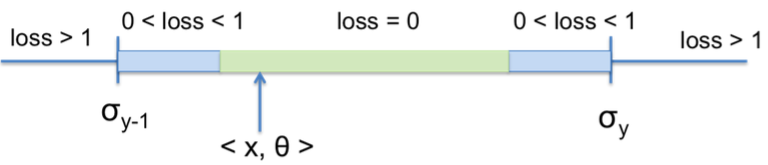
\includegraphics[width=0.8\columnwidth]{ordinal_regression.png}
\end{center}

\subsection{Hinge Loss for Pairwise Ranking}
Applicable when we have only pairwise preferences, e.g. obtained through implicit user feedback:
d is preferred over d$'$ for query q if:\\
\begin{itemize}
  \item d is clicked on, but d$'$ is not clicked on
  \item d$'$ has been presented before d to the user
\end{itemize}

\paragraph{Hinge Loss:}
For preference $d \succ d'$ want $\btheta^{\top} \mathbf{x}_{d, q} > \btheta^{\top} \mathbf{x}_{d', q}$
\begin{align*}
  \underset{\btheta}{\text{arg min}} \; \frac{\lambda}{2}||\btheta||^2 + \frac{1}{n} \sum_{d \succ_q d'} \max\{0, 1 - \btheta^{\top}(\mathbf{x}_{d,q} - \mathbf{x}_{d', q}) \}
\end{align*}

\textcolor{red}{Properties:}
\begin{itemize}
  \item[+] Same problem structure as in binary classification
  \item[--] Many training examples
  \item[--] No focus on ordering at top
\end{itemize}

\subsection{List-Based Ranking}
The idea is to directly maximize a precision-based criterion e.g. (mean) average precision.


%%%%%%%%%%%%%%%%%%%%% Document Indexing %%%%%%%%%%%%%%%%%%%%%%%%%%
\msection{8a - Document Indexing}
\textbf{Index: } An index is an efficient look-up structure for retrieving and scoring documents in real-time. Essential part of any search engine!\\
\textcolor{red}{Advantage:} invest in off-line computation $\Rightarrow$ lower response time, reduce query latency, gain speed-up in processing.

\paragraph{Forward Index:} The processed form of the original document. The processed form can be a tokenized list of terms in the doucment.\\
E.g. Map[doc\_id, List[String]]

\paragraph{Inverted Index:} A data structure that allows to access all occurrences of a given term. E.g. Map[String, List[doc\_id]]

\paragraph{Frequency Index:} Still an inverted index but also with counts. E.g. Map[String, List[(doc\_id, count)]]

\paragraph{Positional Index:} Still an inverted index, but also with position. Often it is important to retain positional information of term occurences. The idea is to create a positional index to score documents higher, which contain the query terms as subsequent terms or in close proximity! \\
E.g. Map[String, List[(doc\_id, position)]]\\
\textcolor{red}{Note:} doc\_id not unique anymore per List!\\
\textcolor{red}{Downside:} Quite expensive positional list intersection required

\paragraph{Indexing Phrases:} Create an inverted index for frequent whole phrases (e.g. 2 or more terms) rather than for single terms! \\
\textcolor{red}{Advantage:} Faster than multi-term indexing via ``Positional Index''\\
\textcolor{red}{Downside:} Requires that we identify phrases at tokenization step!

\paragraph{List Intersection:} A query consists of multiple terms. You often want to retrieve/evaluate only those documents, which contain all terms of a query. This can be achieved efficiently using Inverted Index (if each document list is sorted after doc\_id). For each term we get a document list and hence the task is reduced to List Intersection. \\
\underline{Algorithm:} Iteratively advance pointer of lower doc\_id's until we have a match on all document lists. This allows to work with infinite large streams!

\msection{8b - Index Construction and Serving}
\paragraph{In-Memory Index Construction:} If everything fits in memory then the index can directly be constructed in memory on 1 machine.\\
\textcolor{red}{Issue:} Lack of scalability (speed but also memory)

\paragraph{Blocked Sort-Based Indexing (BSBI):} Create small blocks of postings (e.g. 1 posting = (term\_id, doc\_id, frequency))which fit in memory. Then sort each block (e.g. after term and then doc\_id) and write them to disk. Then merge all blocks into one long sorted order (e.g. external merge sort) and again write to disk. You can then create a dictionary by making one pass over the whole sequence.\\
\underline{Dictionary Representation:}
\begin{enumerate}
  \item Represent token as strings $\Rightarrow$ significant memory blow-up
  \item Maintain global dictionary (String $\Rightarrow$ int)
  \item Token fingerprinting (hashing)
\end{enumerate}

\paragraph{Single-Pass in Memory Indexing (SPIMI):} Don't use a global dictionary (as in BSBI), but partition document collection into sub-collections. Then create an \underline{independent} inverted index for each sub-collection. Then we have 2 options to get the functionality of a global index structure:
\begin{enumerate}
  \item Merge all independent indexes to 1 global index
  \item Run query over all block indexes (merge results)
\end{enumerate}

\paragraph{Distributed Indexing (Map Reduce):} Can use MapReduce to compute global inverted index in a distributed manner.\\
\begin{itemize}
  \item \underline{Mapper:} Each mapper processes one document and generates tuples $<$token, (doc\_id, 1)$>$
  \item \underline{Combiner:} It follows a Mapper and improves performance.\\
        E.g. It can combine duplicate results into $<$token, (doc\_id, tf)$>$
  \item \underline{Reducer:} Gets set of tuples belonging to same key (here token)\\
        E.g. It creates and writes posting lists (token, List[(doc\_id, tf)])
\end{itemize}

\vfill
\columnbreak

%%%%%%%%%%%%%%%%%%%%% Index Serving & Compression %%%%%%%%%%%%%%%%%%%%%%%%%%
\msection{9 - Index Serving \& Compression}
\subsection{Index Serving}
Once index is constructed, then there are still 2 key questions:
\begin{itemize}
  \item Where do we keep index data structure? Memory vs disk
  \item How do we process queries and perform scoring?
\end{itemize}

We have 2 options on how to split up the index into pieces/shards:
\begin{itemize}
  \item \underline{Document sharding:} Each shard contains many short posting lists for a subset of documents.
  \item \underline{Term sharding:} Each shard contains few posting lists for all documents.
\end{itemize}

\paragraph{Document sharding:} We split the posting lists by document ID ranges. Then each shard contains many (1 for every vocabulary term) short posting lists. I.e. for every (term, List[doc\_id]) keep only those doc\_id's which belong to the assigned subset of documents. 
\begin{itemize}
  \item[+] Each shard can process queries independently. I.e. Each shard can compute full scores for each document (not possible in term sharding)
  \item[+] Easy to keep additional per-document information (e.g. tf)
  \item[+] Small network traffic (send query / receive scores) 
  \item[+] Scalable: more documents more shards
  \item[--] Query has to be processed by all N shards
  \item[--] O(K $\cdot$ N) disk seeds for K word query over N shards
\end{itemize}
\begin{center}
  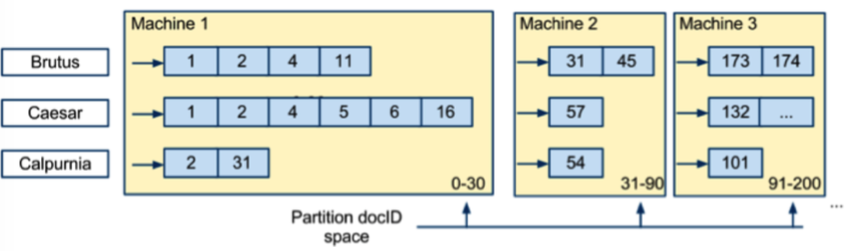
\includegraphics[width=0.9\columnwidth]{document-shard.png}
\end{center}

\paragraph{Term sharding:} We split the index by term ranges. Then each shard contains a few terms, but every term has the full posting lists. I.e. keep full doc\_id's for every (term, List[doc\_id]).
\begin{itemize}
  \item[+] K word query has to be processed by at most K shards
  \item[+] O(K) disk seeds for K word query
  \item[--] Much higher network traffic (need exchange intermediate results)
  \item[--] Data about each term for each matching document must be collected in one place
  \item[--] Harder to have per-document extra information
\end{itemize}
\begin{center}
  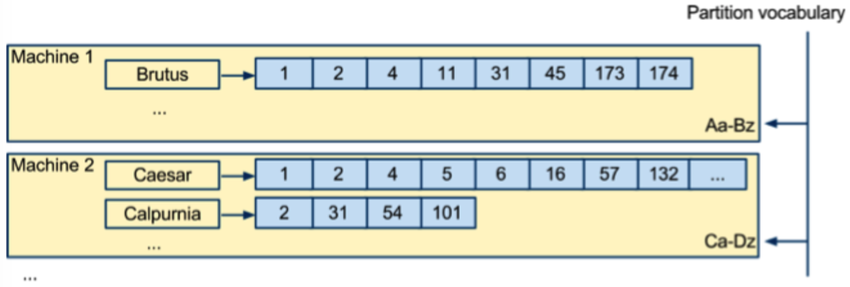
\includegraphics[width=0.9\columnwidth]{term-shard.png}
\end{center}

\subsection{Real-time Scoring}
Makes use of the inverted index.
\paragraph{Distributed Scoring:} Retrieval and scoring is done by shard (in document-sharding). Then need to merge into global result list.

\paragraph{User query:} The query that is issued by the user.
\paragraph{Retrieval query:} The query that we effectively process. We don't want to retrieve documents that are known to have small scores. There are various heuristics that can be used.

\paragraph{Disjunctive retrieval:} Query each term independently and take union of results. This is very conservative and we may retrieve too many documents.

\paragraph{Priority Ordered Posting Lists:} Often we can't scan complete posting lists (because too many documents in it). Hence could order the posting lists (the document\_id's) by their quality (eg PageRank) and then for a query process just the say 1000 first high quality documents. \\
\textcolor{red}{Advantage:} Speed-up, high quality documents are surely considered

\subsection{Dictionary Representation}
\paragraph{Heap's Law:} Estimates the vocabulary (= dictionary) size as a function of the total number of terms in a collection.
\begin{align*}
  \text{Dictionary size: } \text m(n) &= kn^{\beta} \\
  \text{where typically: } \beta &= 0.5 \hspace{0.3cm} \text{and} \hspace{0.3cm}30 \leq k \leq 100
\end{align*}
Here $n$ = \# tokens in collection and for $\beta = 0.5$: m$(n) \in O(\sqrt{n})$\\
\underline{Empirical law:} it behaves linear in log-log space

\textcolor{red}{\textbf{Q:}} Why dictionary (Map[term, $\cdot$]) compression? \\
\textcolor{red}{\textbf{A:}} Want to keep it in memory and also to speed-up startup time.

\paragraph{Fixed-width Array Dictionaries:} Simplest possible dictionary structure. Just keep uncompressed strings with all fixed width fields.
\begin{itemize}
  \item[+] Very easy to implement / work with
  \item[--] waste of space for strings with $<$ 20 characters
  \item[--] can't represent strings with $>$ 20 characters
\end{itemize}
\begin{center}
  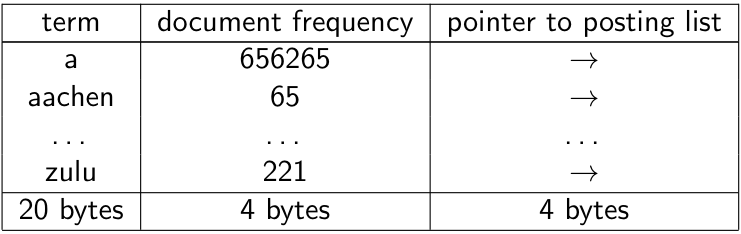
\includegraphics[width=0.6\columnwidth]{dictionary-fixed-width.png}
\end{center}

\paragraph{String Representation for Dictionaries:} Represent dictionary as 1 long String (where all terms are concatenated). Then in the dictionary just store offset to term in the long String. 
\begin{itemize}
  \item[+] Can store arbitrary long Strings (i.e. also $>$ 20 Bytes) 
  \item[+] Saves around 30\% space
  \item[--] Looking up a term is now more complex! (no direct term $\Rightarrow$ posting list pointer)
\end{itemize}
\vspace{-0.5cm}
\begin{center}
  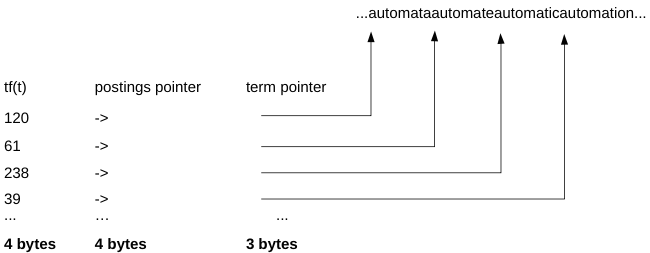
\includegraphics[width=0.7\columnwidth]{dictionary-string-representation.png}
\end{center}

\paragraph{Dictionary Strings with Blocks and Front Coding:} Split the 1 long String into blocks, so that each block contains k terms. Then just maintain pointers to beginning of each block instead of having pointers for each term! Moreover use Front Coding, which replaces common prefix/suffix in a block with special symbols to save space (since many terms have same prefix in lexicographically ordered dictionary e.g. automat /a /ation /ic).
\begin{itemize}
  \item[+] Saves even more space
  \item[--] Tradeoff: compression (larger blocks) vs faster access (smaller blocks)
\end{itemize}

\paragraph{Dictionary via Hash Tables:} Use hash func. to map term to id
\begin{itemize}
  \item[+] Simple and fast
  \item[+] No need to store the Strings (terms)
  \item[+] Most space efficient version
  \item[--] Have to deal with collisions! Either maintain collision list (needs Strings) or use more bytes and live with small collision probabilities!
\end{itemize}
\begin{center}
  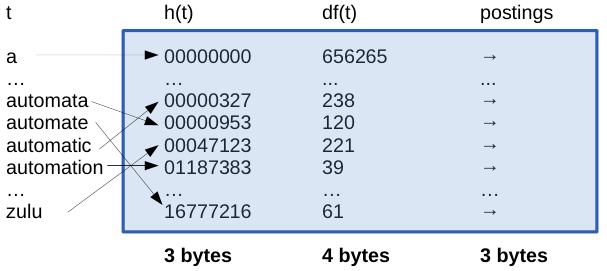
\includegraphics[width=0.7\columnwidth]{dictionary-hash.png}
\end{center}

\subsection{Index Compression}
\paragraph{Zip's Law:} Says that the \underline{collection frequency} of the $i$-th word cf$_i$ is proportional to $1/i$. Note w$_i$ corresponds to the $i$-th most frequent word in the collection.
\begin{align*}
  \text{collection frequency: } \text{cf}_i \propto \frac{1}{i} \Leftrightarrow \log \text{cf}_i = - \log i + \text{const}
\end{align*}
\textcolor{red}{Important is only:} Few frequent terms and many rare terms!

\paragraph{Gap Encoding:} Tries to compress the document ID's in posting lists. The idea is to \underline{encode the gap} between doc\_id's instead of the doc\_id itself, since the gap is often smaller and thus saves space!

\paragraph{Variable Length Encoding:} We want to spend fewer bits for small numbers (for gaps), since they occur more often! This requires a variable length encoding. \\
\begin{addmargin}[0.28cm]{0cm} % left, right
  \underline{Variable Byte Code:} Number of bits: always multiple of 8 (1 Byte)
  \begin{itemize}
    \item Use 7 bits to encode number
    \item Use 1 bit as continuation bit (1 = stop, 0 = continue)
  \end{itemize}
  \textcolor{red}{Advantages:} Extremely simple \& efficient to implement\\
  \textcolor{red}{Limitation:} Code length always multiple of 8 bits\\
  \textcolor{red}{Note:} For numbers $\geq$ 128 need at least 2 Bytes!\\
  \underline{Examples:}
  \begin{align*}
    3   &\Rightarrow& \hspace{-2cm} \textcolor{red}{1}0000011& \\
    127 &\Rightarrow& \hspace{-2cm} \textcolor{red}{1}1111111& \\
    130 &\Rightarrow& \hspace{-2cm} \textcolor{red}{0}0000001 \hspace{0.1cm} \textcolor{red}{1}0000010& 
  \end{align*}
\end{addmargin}
\begin{tabular}{l|r|r|r|r|r|r|r|r|r|r|r}
  \text{Bit} & 11 & 10 & 9 & 8 & 7 & 6 & 5 & 4 & 3 & 2 & 1 \\
  \hline    
  \text{Bin} & $2^{10}$ & $2^9$ & $2^8$ & $2^7$ & $2^6$ & $2^5$ & $2^4$ & $2^3$ & $2^2$ & $2^1$ & $2^0$ \\
  \hline
  \text{Num} & 1024 & 512 & 256 & 128 & 64 & 32 & 16 & 8 & 4 & 2 & 1
\end{tabular} 

\paragraph{Gamma Code:} Also wants to spend fewer bits for small numbers, but uses bit level control over codeword length (unlike VB Code where it was on byte level). Gamma codes are prefix codes!\\
\textcolor{red}{Note:} VB Code is preferred in general!
\begin{itemize}
  \item[+] Higher compression then VB Code
  \item[--] Machines typically have 8, 16, 32 word boundaries
  \item[--] VB Code alignment potentially more efficient (always 8 bit)
  \item[--] VB Code conceptually simpler with just little space overhead
\end{itemize}
\vspace{0.2cm}
\begin{addmargin}[0.28cm]{0cm} % left, right
  \underline{Gamma Code:} Encode number n as bit strings: length and offset
  \begin{itemize}
    \item offset = binary representation of n with leading 1 removed
    \item length = unary code for number of bits in offset with tailing 0
    \item concatenate: length + offset
  \end{itemize}
  \underline{Encode ex.:}\\
  \vspace{-0.3cm}
  \begin{flushright}
    \begin{tabular}{r|r|r|r|r}
      num & bin & offset & length & $\gamma$-code \\
      \hline
      0 & 0 & - & - & - \\
      1 & 1 & - & 0 & 0, \\
      2 & 10 & 0 & 10 & 10,0\\
      42 & 101010 & 01010 & 111110 & 111110,01010\\
    \end{tabular}
  \end{flushright}
  \underline{Decode ex.:}\\
  \vspace{-0.3cm}
  \hspace{2cm}
    \begin{tabular}{r|r|r}
      $\gamma$-code & bin & num\\
      \hline
      0, & 1 & 1 \\
      10,0 & 10 & 2\\
      111110,01010 & 101010 & 42
    \end{tabular}    \\
    \textcolor{red}{Attention:} To interpret code must prepend 1 to offset!\\
  \textbf{Q:} What is length of bits in $\gamma$-code of n $\in \N$? \textbf{A:} $2 \log(n) - 1$ 
\end{addmargin}

\paragraph{Golomb Code:} For term frequencies with a geometric distribution one can create ``optimal'' Huffmann style codes called Golomb Codes! Optimal in the sense that more frequent terms have shorter codes and vice versa. \\
\textcolor{red}{Note:} Golomb Code would be best in terms of compression, but not only that matters!
\begin{addmargin}[0.28cm]{0cm} % left, right
  \underline{Golomb Code:} Encode number $x \geq 1$ given parameter b:
  \begin{itemize}
    \item Compute quotient: $q = \lfloor (x-1)/b \rfloor$
    \item Compute remainder: $r = (x-1) \mod b$
    \item Encode $q$ in unary ($q \times 1$ + 0) followed by $r$ in binary
  \end{itemize}
  \underline{Encode ex:}
  \begin{align*}
    \text{Given: } &b = 4 \text{ and } x = 15 \\
                   &\Rightarrow q = \lfloor 14 / 4 \rfloor = 3 &&\Rightarrow 1110\\
                   &\Rightarrow r = 14 \mod b = 2 &&\Rightarrow 10 \\
                   &\Rightarrow 111010
  \end{align*}
  \underline{Decode ex:} $q \cdot b$ + $r$ + 1
  \begin{align*}
    \text{Given: } &b = 4, q = 3 \text{ and } r = 2 \\
                  &\Rightarrow 3 \cdot 4 + 2 + 1 = 15
  \end{align*}
\end{addmargin}

\paragraph{Group Varint Encoding:} Golomb Codes or Block-Based Index Formats have good compression, but are expensive to decode. Group Varint Encoding is more efficient! The idea is to put $4 \times 2$ bit lengths together in 1 Byte! Now encoding is limited to 32 bits. The 2 bits encode how many bytes (1-4) have to be read!

\msection{Convex Optimization}
\textbf{Primal problem:} 
$ \min_{\textbf{x}} f(\mathbf{x}) \quad \text{subject to} \quad g_i(\mathbf{x}) \leq 0, i = 1, \ldots, m$\\
\hspace{6.6cm} $h_i(\mathbf{x}) = 0, i = 1, \ldots, p$\\
\textbf{Lagrangian:} 
$L(\mathbf{x}, \lambda, \nu) \hspace{-0.05cm} = \hspace{-0.05cm} f(\mathbf{x}) + \hspace{-0.1cm} \sum\limits_{i=1}^m \lambda_i g_i(\mathbf{x}) + \hspace{-0.1cm} \sum\limits_{i=1}^p \nu_i h_i(\mathbf{x})$ where $\lambda \hspace{-0.05cm} \geq \hspace{-0.05cm} 0$\\
\textbf{Dual function:}
$d(\lambda, \nu) = \inf\limits_\textbf{x} L(\mathbf{x}, \lambda, \nu)$\\
\textbf{Dual problem:}
$\max\limits_{\lambda, \nu} \; d(\lambda, \nu) \quad \text{subject to} \quad \lambda \geq 0$\\
\textbf{Recover optimal \textbf{x}}: $\textbf{x}^\star = \argmin_\mathbf{x} L(\textbf{x}, \lambda^\star, \nu^\star)$

\textbf{Note:} Dual function is a lower bound on optimal value $p^\star$ of primal!\\
\emph{Proof:} $d(\lambda, \nu) = \inf\limits_{\mathbf{x}} L(\mathbf{x}, \lambda, \nu) \leq  
\inf\limits_{\tilde{\mathbf{x}}} L(\tilde{\mathbf{x}}, \lambda, \nu) \leq
\min\limits_{\tilde{\mathbf{x}}} f(\mathbf{\tilde{x}}) = p^\star$


\subsection{Convex optimization with equality constraints}
\textbf{Primal problem:} $\min_{x} f(x) \quad \text{subject to} \quad Ax = b$\\
\textbf{Lagrangian:} $L(\mathbf{x}, \nu) = f(x) + \nu^\top(A x - b)$\\
\textbf{Dual function:} $d(\nu) = \inf_x L(x, \nu)$\\
\textbf{Dual problem:} $\max\limits_{\nu} \; d(\nu)$\\

\underline{\textbf{Gradient Method for dual:}}\\
\hspace{0.2cm}$x^{k+1} = \argmin_x L(x, \nu^k)$ \\
\hspace{0.2cm}$\nu^{k+1} \hspace{-0.05cm} = \hspace{-0.05cm} \nu^{k} \hspace{-0.05cm} + \hspace{-0.05cm} \alpha^k \nabla d(\nu^k) \hspace{-0.05cm} = \hspace{-0.05cm} \nu^{k} \hspace{-0.05cm} + \hspace{-0.05cm} \alpha^k \frac{\partial}{\partial \nu} L(x^{k+1}, \nu^{k}) \hspace{-0.05cm} = \hspace{-0.05cm} \nu^{k} \hspace{-0.05cm} + \hspace{-0.05cm} \alpha^k (A x^{k+1} - b)$\\

\underline{\textbf{Dual decomposition:}} If $f(x)$ with $x \in \R^n$ is separable than $L(x, \nu)$ is separable and we can split the x-min step:
\\
$f(x) = f_1(x_1) + ... + f_n(x_n) \Rightarrow L(x, \nu) = L_1(x_1, \nu) + ... + L_n(x_n, \nu) - \nu^\top b$\\
\hspace{0.2cm}$x_i^{k+1} = \argmin_{x_i} L_i(x_i, \nu^k) = \argmin_{x_i} f_i(x_i) + \nu^\top A_i x_i \quad i=1..n$ \\
\hspace{0.2cm}$\nu^{k+1} = \nu^{k} + \alpha^k \nabla d(\nu^k) = \nu^{k} + \alpha^k (\sum_{i=1}^n A_i x_i^{k+1} - b)$

\underline{\textbf{Method of Multipliers:}} Augment Lagrangian to $L_\rho$ with ${\rho \over 2} ||\cdot||_2^2$\\
$L_\rho (x,\nu) = f(x) + \nu^T (Ax-b) + {\rho \over 2} ||Ax-b||_2^2$\\
\hspace{0.2cm}$x^{k+1} = \argmin_x L_\rho (x,\nu^k)$\\
\hspace{0.2cm}$\nu^{k+1} = \nu^k + \rho \nabla d(\nu^k) = \nu^k + \rho (Ax^{k+1}-b)$\\

Choose $\rho$ as step size, since $x^{k+1}$ minimizes $L_\rho(x, \nu^k)$:
\[
 0 =\nabla_x L\rho(x^{k+1}, \nu^k) = \nabla_x f(x^{k+1}) + \underbrace{A^T (\nu^k +\rho(Ax^{k+1}-b))}_{A^T \nu^{k+1}}
\]

\underline{\textbf{Alternating Direction Method of Multipliers:}}\\
Since aug. Lag. $L_\rho$ not separable anymore, can't parallelize x-min!\\
Primal: $\min_{x, z} f(x) + p(z)\ \text{ subject to }\ Ax+Bz = c \quad f,p \text{ convex}$\\
$L(x, z, \nu) = f(x) + p(z)+ \nu^T (Ax+Bz-c)$\\
$L_\rho(x, z, \nu) = f(x) + p(z)+ \nu^T (Ax+Bz-c) + {\rho \over 2}||Ax + Bz- c||_2^2$\\
\hspace{0.2cm}$x^{k+1} = \argmin_x L_\rho (x, z^k, \nu^k)$\\
\hspace{0.2cm}$z^{k+1} = \argmin_z L_\rho(x^{k+1}, z, \nu^k)$\\
\hspace{0.2cm}$\nu^{k+1} = \nu^k + \rho \nabla d(\nu^k) = \nu^k + \rho(Ax^{k+1}+Bz^{k+1}-c)$\\
Primal Feasibility condition: $Ax^\star + Bz^\star - c = 0$\\
Dual Feasibiliy conditions:$\nabla f(x^\star) \hspace{-0.05cm} + \hspace{-0.05cm} A^\top \nu^\star \hspace{-0.05cm} = \hspace{-0.05cm} 0$ and $\nabla p(z^\star) \hspace{-0.05cm} + \hspace{-0.05cm} B^\top \nu^\star \hspace{-0.05cm} = \hspace{-0.05cm} 0$
\end{multicols}%}
\end{document}